%%%%%%%%%%%%%%%%%%%%%%%%%%%%%%%%%%%%%%%%%
% AOS Masters Thesis 
% LaTeX Template
% Version 0.1 (04/08/16)
%
% A derivation of the thesis template from www.latextemplates.com.
%
% AOS customization:
% Ethan Nelson
% http://github.com/ethan-nelson/AOSthesis-template
%
% Original authors:
% Steven Gunn 
% http://users.ecs.soton.ac.uk/srg/softwaretools/document/templates/
% and
% Sunil Patel
% http://www.sunilpatel.co.uk/thesis-template/
%
% License:
% CC BY-NC-SA 3.0 (http://creativecommons.org/licenses/by-nc-sa/3.0/)
%
% Note:
% Make sure to edit document variables in the Thesis.cls file
%
%%%%%%%%%%%%%%%%%%%%%%%%%%%%%%%%%%%%%%%%%

%----------------------------------------------------------------------------------------
%	PACKAGES AND OTHER DOCUMENT CONFIGURATIONS
%----------------------------------------------------------------------------------------

\documentclass[12pt,letterpaper,oneside]{Thesis}
\usepackage{titlesec}
\usepackage{multirow}
\usepackage{hhline}
\titlespacing{\section}{0pt}{0pt}{-0.35cm}
\titlespacing{\subsection}{0pt}{0pt}{-0.35cm}

\usepackage{afterpage}
\usepackage{pdflscape}
\usetikzlibrary{shapes.arrows,fadings}

\usepackage[comma, sort&compress]{natbib}
\hypersetup{colorlinks=false}
\title{\ttitle}

\begin{document}

\frontmatter 

\setstretch{1.5} % Line spacing of 1.3

\fancyhead{} % Clears all page headers and footers
\rhead{\thepage} % Sets the right side header to show the page number
\lhead{}

\pagestyle{fancy}

\newcommand{\HRule}{\rule{\linewidth}{0.5mm}}

% PDF meta-data
\hypersetup{pdftitle={\ttitle}}
\hypersetup{pdfauthor=\authornames}

\makeatletter
\renewcommand\chapter{\if@openright\cleardoublepage\else\clearpage\fi
                    \thispagestyle{fancy}%
                    \global\@topnum\z@
                    \@afterindentfalse
                    \secdef\@chapter\@schapter}
\makeatother

%----------------------------------------------------------------------------------------
%	TITLE PAGE
%----------------------------------------------------------------------------------------

\begin{titlepage}
\begin{center}

\HRule \\[0.4cm] % Horizontal line
\setstretch{3}
{\huge \bfseries \ttitle}\\[0.4cm] % Thesis title
\setstretch{1.8}
\HRule \\[1.5cm] % Horizontal line

\begin{center} \large
\authornames 
\end{center}
 
\large A thesis submitted in partial fulfillment of \\ the requirements for the degree of\\[1cm]
\degreename \\
(\subjectname) \\[1cm]
 at the\\
\textsc{\univname}\\
{\large \graduationmonth \ \graduationyear}\\[4cm] % Date
%\includegraphics{Logo} % University/department logo - uncomment to place it
 
\vfill
\end{center}

\end{titlepage}

%----------------------------------------------------------------------------------------
%	DECLARATION PAGE
%----------------------------------------------------------------------------------------

\thispagestyle{empty}
\Declaration{
\thispagestyle{empty}

\newcommand{\sigline}[3]{\leavevmode\vtop{\vbox{\hbox{\text{#2}}\smallskip}\hrule width #1\smallskip\hbox{#3}}}

I, \authornames, declare that this thesis titled `\ttitle' and the work presented in it are my own.

\vfill

\sigline{1.8in}{\authornames\phantom{g}}{Author}\hfill\sigline{2.5in}{}{Signature}\hfill\sigline{1in}{}{Date}

\vfill

I hereby approve and recommend for acceptance this work in partial fulfillment of the requirements for the degree of \degreename:

\vfill

\sigline{1.8in}{\committeenameone\phantom{g}}{\committeeroleone}\hfill\sigline{2.5in}{}{Signature}\hfill\sigline{1in}{}{Date}

\vfill

\sigline{1.8in}{\committeenametwo\phantom{g}}{\committeeroletwo}\hfill\sigline{2.5in}{}{Signature}\hfill\sigline{1in}{}{Date}

\vfill

\sigline{1.8in}{\committeenamethree\phantom{g}}{\committeerolethree}\hfill\sigline{2.5in}{}{Signature}\hfill\sigline{1in}{}{Date}

\vfill

}
\clearpage



%----------------------------------------------------------------------------------------
%	ABSTRACT PAGE
%----------------------------------------------------------------------------------------
\setstretch{2}
\addtotoc{Abstract} % Add the "Abstract" page entry to the Contents
\addtocounter{page}{-1}

\abstract{

The atmosphere is a crucial part of everyday life by providing biological matter to respirate. Other planets in our solar system are characterized by a lack of atmosphere and thus remain unsuitable for life. Modeling a planet with no atmosphere resolves many of the issues plagued by modellers, especially pertaining to the issue of magnitudes of scales.

}

\clearpage % Start a new page

%%----------------------------------------------------------------------------------------
%%	QUOTATION PAGE
%%----------------------------------------------------------------------------------------

\pagestyle{empty} % No headers or footers for the following pages

\null\vfill % Add some space to move the quote down the page a bit

\textit{``Thanks to my solid academic training, today I can write hundreds of words on virtually any topic without possessing a shred of information, which is how I got a good job in journalism."}

\begin{flushright}
Dave Barry
\end{flushright}

\vfill\vfill\vfill\vfill\vfill\vfill\null % Add some space at the bottom to position the quote just right

\clearpage % Start a new page

%----------------------------------------------------------------------------------------
%	DEDICATION
%----------------------------------------------------------------------------------------

\setstretch{1.3} % Return the line spacing back to 1.3
\addtotoc{Dedication}
\pagestyle{empty} % Page style needs to be empty for this page

\dedicatory{This work is dedicated to the love of my life, Python.} % Dedication text


%----------------------------------------------------------------------------------------
%	ACKNOWLEDGEMENTS
%----------------------------------------------------------------------------------------

\setstretch{1.5} % Reset the line-spacing to 1.3 for body text (if it has changed)

\acknowledgements{

There are many people that made this possible. 

First, my advisor advised me very well.

Second, my colleagues and flatmates were very collegial.

Finally, my mom and dad have been parental to me.

Thanks to the data repository for providing data used in this thesis.

Acknowledgement is also made to the Department of Research for support under grants \#1, 5, and 290. 

}
\clearpage % Start a new page

%----------------------------------------------------------------------------------------
%	LIST OF CONTENTS/FIGURES/TABLES PAGES
%----------------------------------------------------------------------------------------

\pagestyle{fancy} % The page style headers have been "empty" all this time, now use the "fancy" headers as defined before to bring them back

\begingroup
\lhead{\emph{Contents}} % Set the left side page header to "Contents"
\tableofcontents % Write out the Table of Contents

\lhead{\emph{List of Figures}} % Set the left side page header to "List of Figures"
\listoffigures % Write out the List of Figures

\lhead{\emph{List of Tables}} % Set the left side page header to "List of Tables"
\listoftables % Write out the List of Tables
\endgroup
%----------------------------------------------------------------------------------------
%	ABBREVIATIONS
%----------------------------------------------------------------------------------------

\clearpage % Start a new page

%\setstretch{1.5} % Set the line spacing to 1.5, this makes the following tables easier to read

\lhead{\emph{\listabbreviationname}} % Set the left side page header to "Abbreviations"
\listofabbreviations{ll} % Include a list of Abbreviations (a table of two columns)
{

%\textbf{Acronym} & \textbf{W}hat (it) \textbf{S}tands \textbf{F}or \\
\textbf{CPR} & \textbf{C}loud \textbf{P}rofiling \textbf{R}adar (aboard CloudSat) \\
\textbf{MJO} & \textbf{M}adden-\textbf{J}ulian Oscillation \\
\textbf{TRMM} & \textbf{T}ropical \textbf{R}ainfall \textbf{M}easuring \textbf{M}ission 
}

%----------------------------------------------------------------------------------------
%	PHYSICAL CONSTANTS/OTHER DEFINITIONS
%----------------------------------------------------------------------------------------

\clearpage % Start a new page

\lhead{\emph{Physical Constants}} % Set the left side page header to "Physical Constants"

\listofconstants{lrcl} % Include a list of Physical Constants (a four column table)
{
Speed of Light & $c$ & $=$ & $2.997\ 924\ 58\times10^{8}\ \mbox{ms}^{-\mbox{s}}$ (exact)\\
% Constant Name & Symbol & = & Constant Value (with units) \\
}

%----------------------------------------------------------------------------------------
%	SYMBOLS
%----------------------------------------------------------------------------------------

\clearpage % Start a new page

\lhead{\emph{Symbols}} % Set the left side page header to "Symbols"

\listofnomenclature{lll} % Include a list of Symbols (a three column table)
{
$a$ & distance & m \\
$P$ & power & W (Js$^{-1}$) \\
% Symbol & Name & Unit \\

& & \\ % Gap to separate the Roman symbols from the Greek

$\omega$ & angular frequency & rads$^{-1}$ \\
% Symbol & Name & Unit \\
}


%----------------------------------------------------------------------------------------
%	THESIS CONTENT - CHAPTERS
%----------------------------------------------------------------------------------------

\mainmatter % Begin numeric (1,2,3...) page numbering
\setstretch{2.0}
\pagestyle{fancy} % Return the page headers back to the "fancy" style

% Include the chapters of the thesis as separate files from the Chapters folder
% Uncomment the lines as you write the chapters

% Chapter 1

\chapter{Introduction} % Chapter title

\label{Chapter1} % Change X to a consecutive number; for referencing this chapter elsewhere, use \ref{ChapterX}

%----------------------------------------------------------------------------------------
%	Chapter text below
%----------------------------------------------------------------------------------------

\section{Preface}\label{section:preface}
This is \sref{section:preface} that provides all of the information about my background. Be sure to check out \ssref{subsection:postscript} as well for more information. Please find \fref{atrain} for more information.

\subsection{Preface Postscript}\label{subsection:postscript}
Sometimes it is necessary to provide information about the background in segments.

\subsection{Postpostscript}

\begin{figure}[h]
\centering
	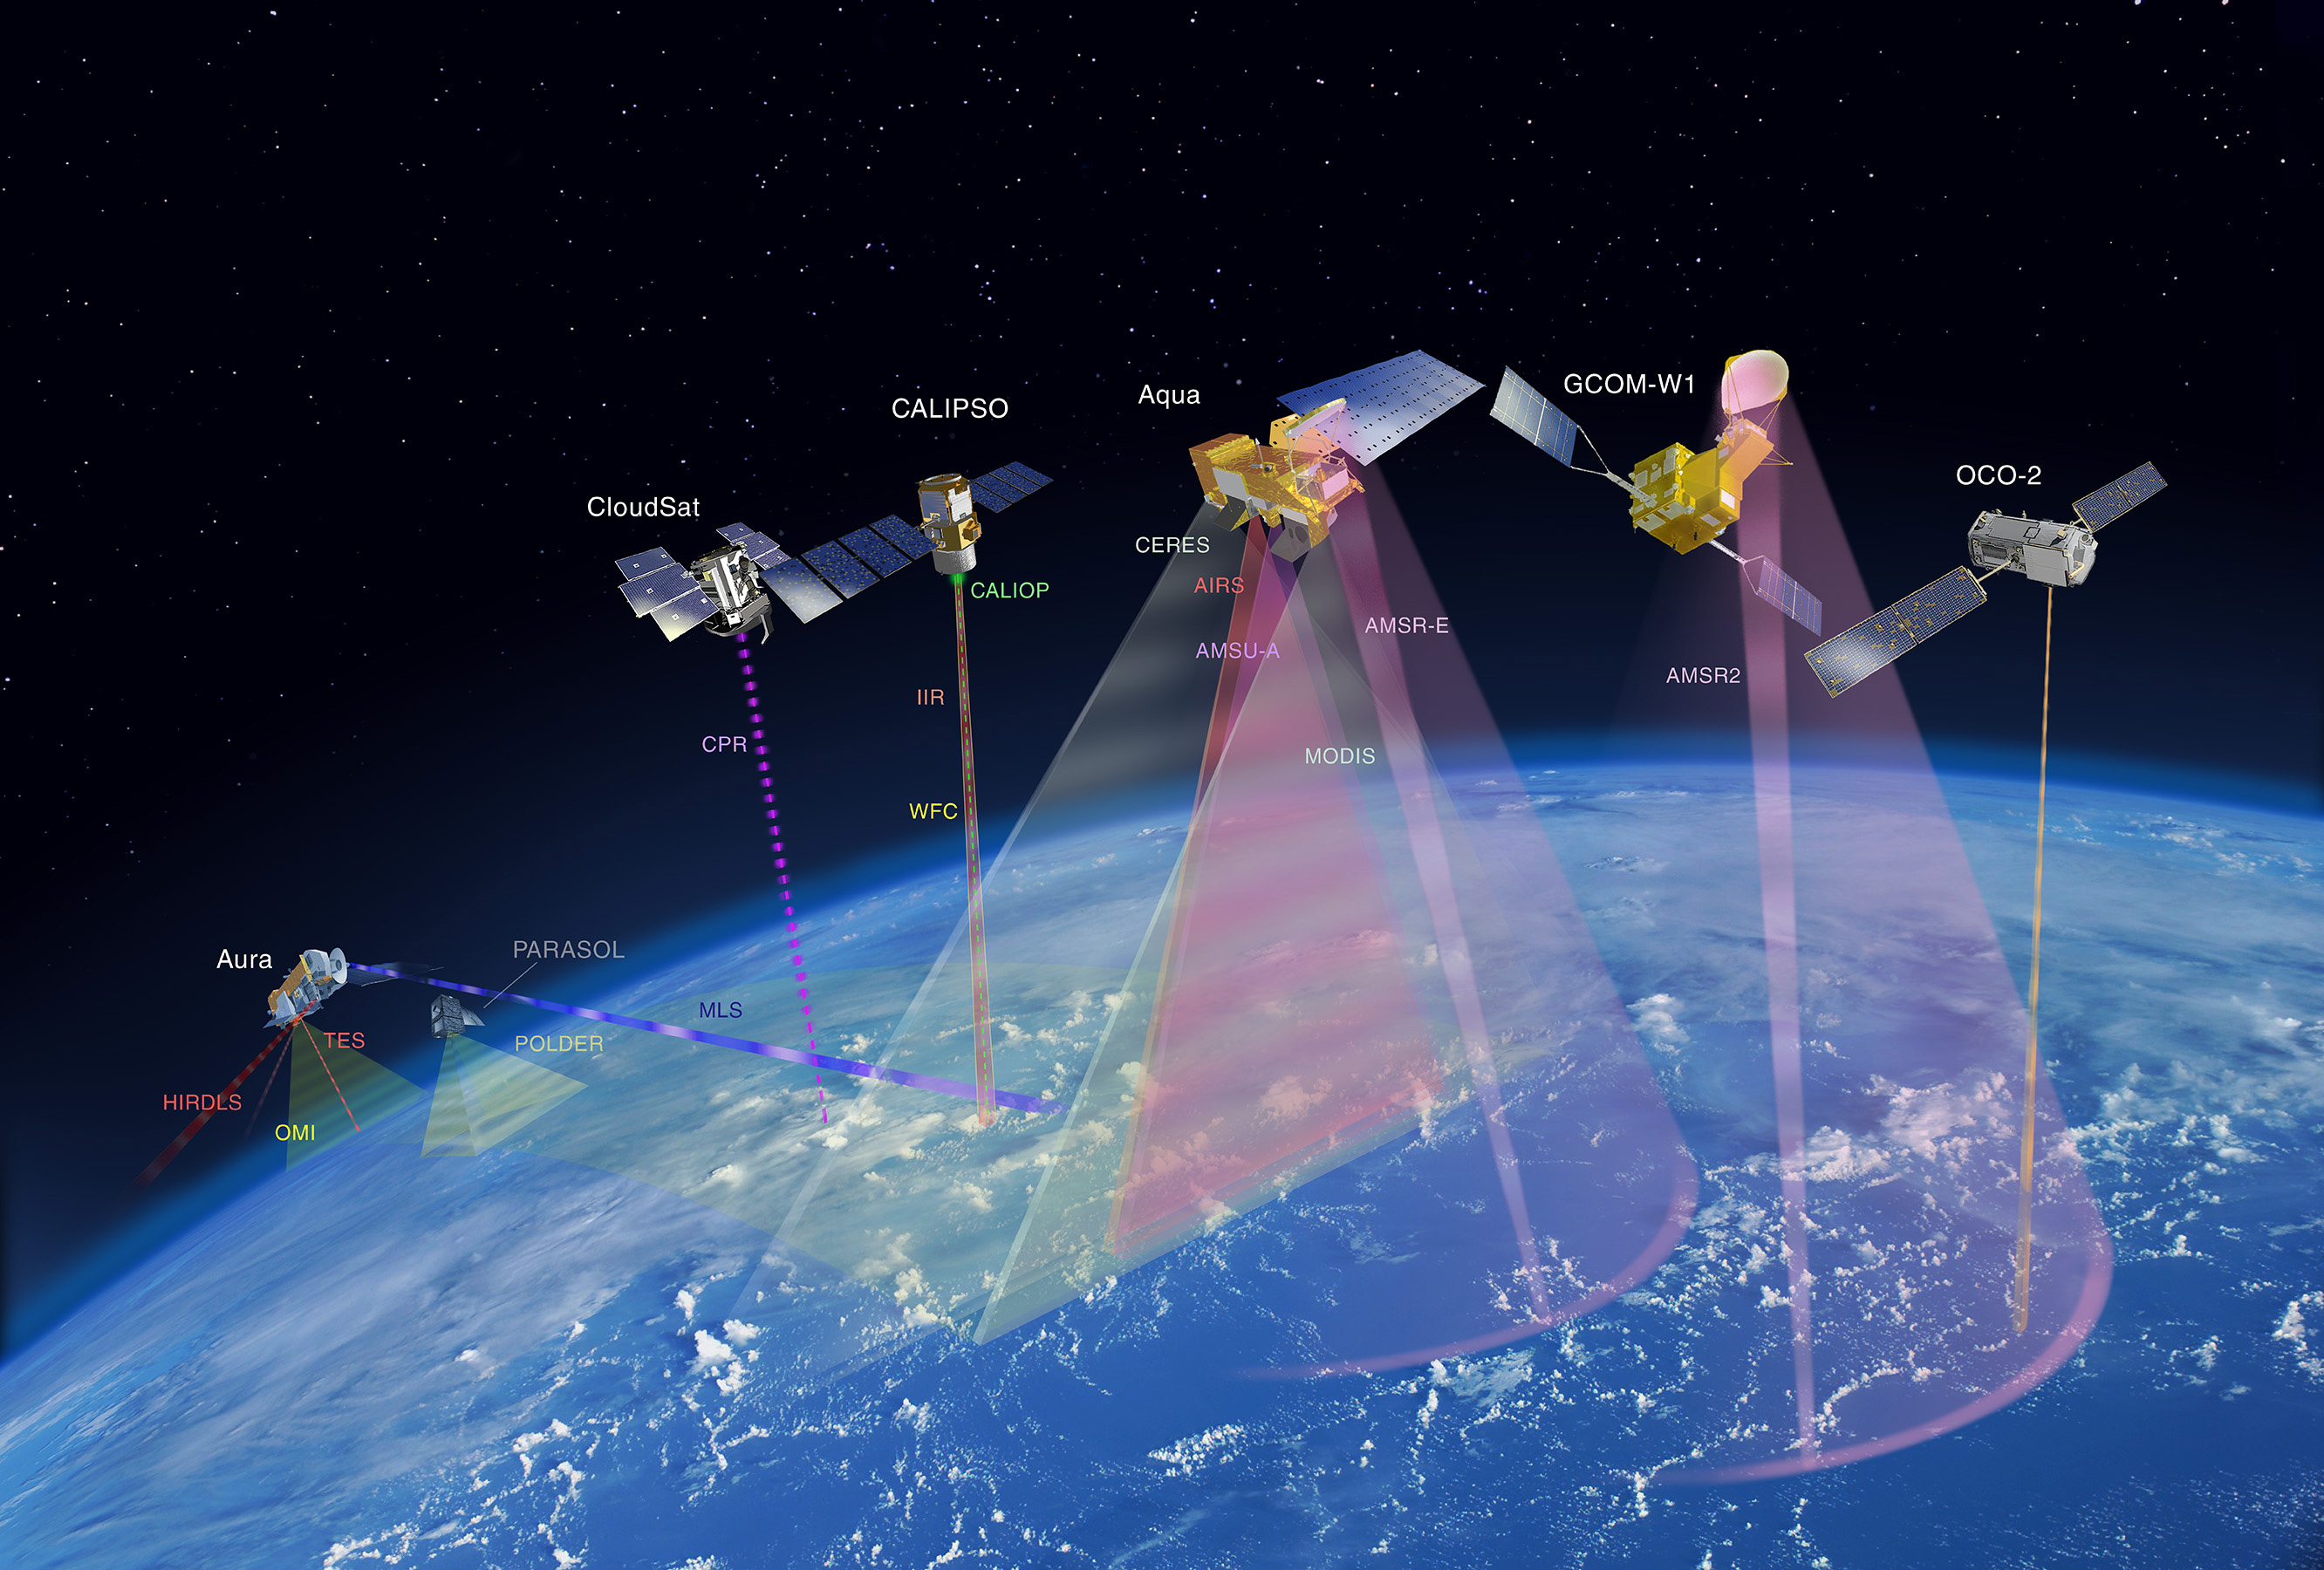
\includegraphics[width=0.6\linewidth]{Figures/atrain.jpeg}
	\rule{35em}{0.5pt}
	\caption[Afternoon Constellation illustration]{An illustration of the Afternoon Constellation (A-Train) satellite mission of NASA with the satellites' respective instruments. CloudSat is second from the left. Illustration courtesy of NASA.}\label{atrain}
\end{figure}

Other areas of interest.

Blah

Blah

\begin{table}[h]
    \centering
    \begin{tabular}{l|l|l}
    ~          & Header 1 & Header 2 \\ \hline \hline
    Category 1 & Data 11  & Data 21  \\ \hline
    Category 2 & Data 12  & Data 22  \\
    \end{tabular}
    \rule{35em}{0.5pt}
    \caption[Short title here.]{We have some data here.}
\end{table}

\begin{itemize}
\item In case you don't know \LaTeX{}
\end{itemize}

\begin{enumerate}
\item \citet{Tanelli2008} is relevant to the material at hand \cite{Tanelli2008}.
\end{enumerate}
%\input{Chapters/Chapter2} 
%\input{Chapters/Chapter3}
%\input{Chapters/Chapter4} 
%\input{Chapters/Chapter5} 
%\input{Chapters/Chapter6} 

%----------------------------------------------------------------------------------------
%	THESIS CONTENT - APPENDICES
%----------------------------------------------------------------------------------------

\addtocontents{toc}{\vspace{2em}} % Add a gap in the Contents, for aesthetics

\appendix % Cue to tell LaTeX that the following 'chapters' are Appendices

% Include the appendices of the thesis as separate files from the Appendices folder
% Uncomment the lines as you write the Appendices

% Appendix A

\chapter{Appendix of Information} % Main appendix title

\label{AppendixA} % For referencing this appendix elsewhere, use \ref{AppendixA}

\lhead{Appendix A. \emph{Appendix of Information}} % This is for the header on each page - perhaps a shortened title

Here's information about stuff that isn't necessary in the regular chapters, but should be in the appendix.
%\input{Appendices/AppendixB}
%\input{Appendices/AppendixC}

\addtocontents{toc}{\vspace{2em}} % Add a gap in the Contents, for aesthetics

\backmatter

%----------------------------------------------------------------------------------------
%	BIBLIOGRAPHY
%----------------------------------------------------------------------------------------

\label{References}

\lhead{\emph{References}} % Change the page header to say "Bibliography"

\bibliographystyle{ametsoc} % Use the "unsrtnat" BibTeX style for formatting the Bibliography

\bibliography{Bibliography} % The references (bibliography) information are stored in the file named "Bibliography.bib"

\end{document}  
